\documentclass[11pt]{exam}
\usepackage[utf8]{inputenc}
\usepackage{hyperref}
\usepackage{graphicx}

\title{Reglas de Asociación en Weka}
\author{Laura Rodríguez Navas \\ rodrigueznavas@posgrado.uimp.es}
\date{\today}

\pagestyle{plain}

\begin{document}

\maketitle

En esta práctica se realiza un estudio acerca de los datos del hundimiento del Titanic a través de la herramienta \href{https://www.cs.waikato.ac.nz/ml/weka/}{Weka}. Los datos se encuentran en la dirección \url{http://www.hakank.org/weka/titanic.arff} y corresponden a las características de los 2201 pasajeros del Titanic. Estos datos son reales y se han obtenido de \textit{"Report on the Loss of the 'Titanic' (S.S.)" (1990), British Board of Trade Inquiry Report\_(reprint), Gloucester, UK: Allan Sutton Publishing}.

\vspace{3mm}

Para realizar esta práctica, se debe cargar el dataset Titanic que se ha descargado anteriormente y contestar a las siguientes preguntas:

\begin{questions}

% Pregunta 1
{\question Cuando ejecutamos el algoritmo Apriori de Weka, podemos utilizar diferentes umbrales de soporte. Dependiendo de qué umbrales de soporte pongamos, nos saldrán más o menos itemsets. Como resultado, Weka nos proporciona un conjunto de ítems L(1)... L(4) cuyos números van variando conforme cambiamos el umbral de soporte. 
	
Responde a las siguientes preguntas, utilizando capturas de pantalla y explicando los resultados de manera clara y concisa:}

\begin{parts}
\part ¿Qué representan cada uno de estos conjuntos de ítems? 

\renewcommand{\figurename}{Figura}

\begin{figure}[h]
	\centering
	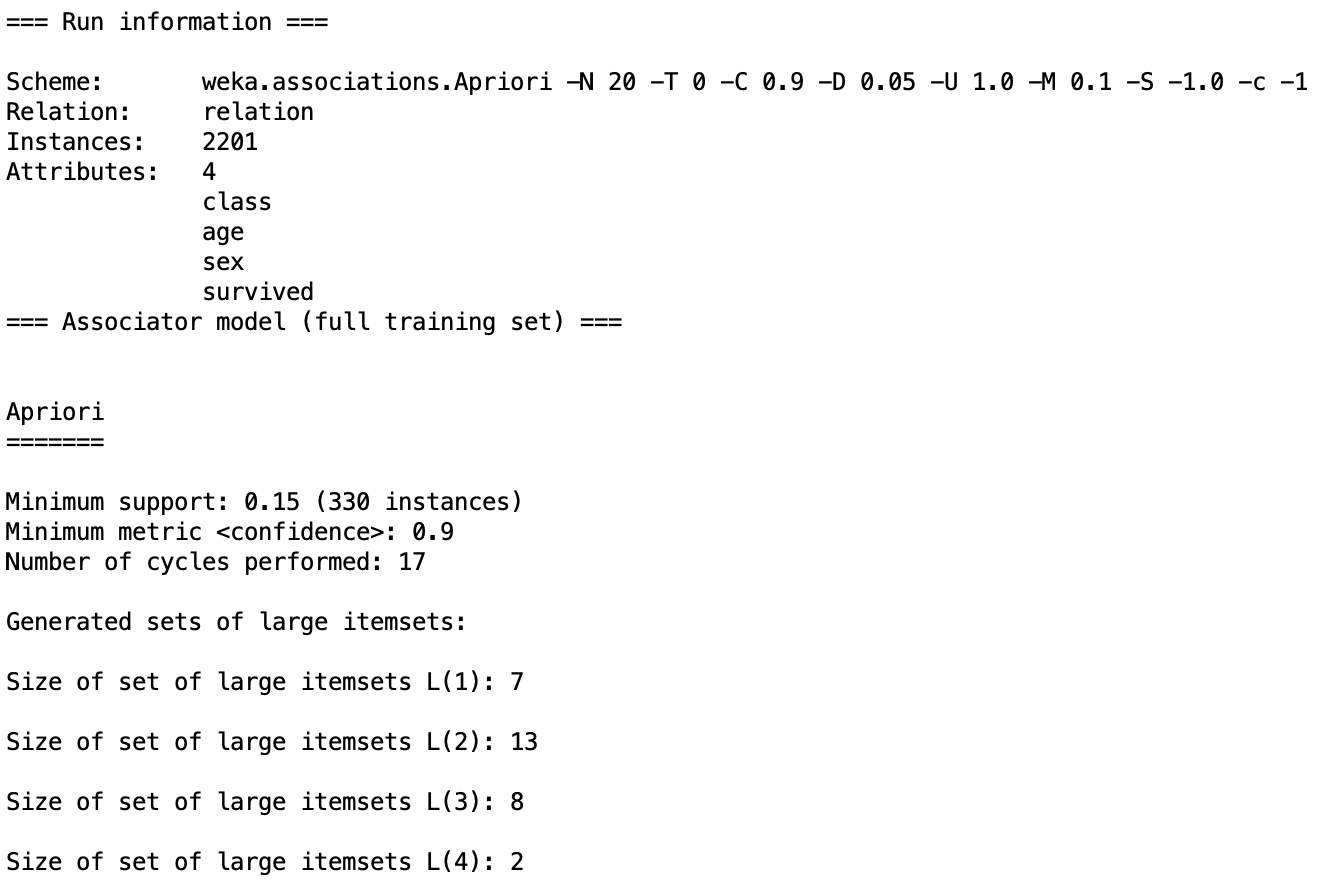
\includegraphics[scale=0.5]{Captura_1_1.png}
	\caption{soporte = 0.15 y confianza = 0.9.}
	\label{Captura_1_1}
\end{figure}

\begin{enumerate}
	\item El conjunto de ítems L(1) representa el número de conjuntos de ítems de tamaño 1 encontrados en el dataset. Que en este caso son 7.
	\item El conjunto de ítems L(2) representa el número de conjuntos de ítems de tamaño 2 encontrados en el dataset. Que en este caso son 13.
	\item El conjunto de ítems L(3) representa el número de conjuntos de ítems de tamaño 3 encontrados en el dataset. Que en este caso son 8.
	\item El conjunto de ítems L(4) representa el número de conjuntos de ítems de tamaño 4 encontrados en el dataset. Que en este caso son 2.
\end{enumerate}	

\part ¿Puede existir L(0)? Explica porqué.

No puede existir L(0). El conjunto de ítems L(0) representa el número de conjuntos de ítems de tamaño 0, es decir, el número de conjuntos de ítems vacíos, y el conjunto vacío (\{$\emptyset$\}) no es válido como conjunto de ítems.

\part ¿Puede existir L(5)? Explica porqué.

No pueden existir conjuntos de ítems de tamaño 5 porqué en el dataset de Titanic no hay un atributo que tenga 5 valores. Como máximo hay un atributo que tiene 4 valores. Este atributo es el atributo Class (ver Figura \ref{Captura_1_2}). 

\begin{figure}[h]
	\begin{center}
		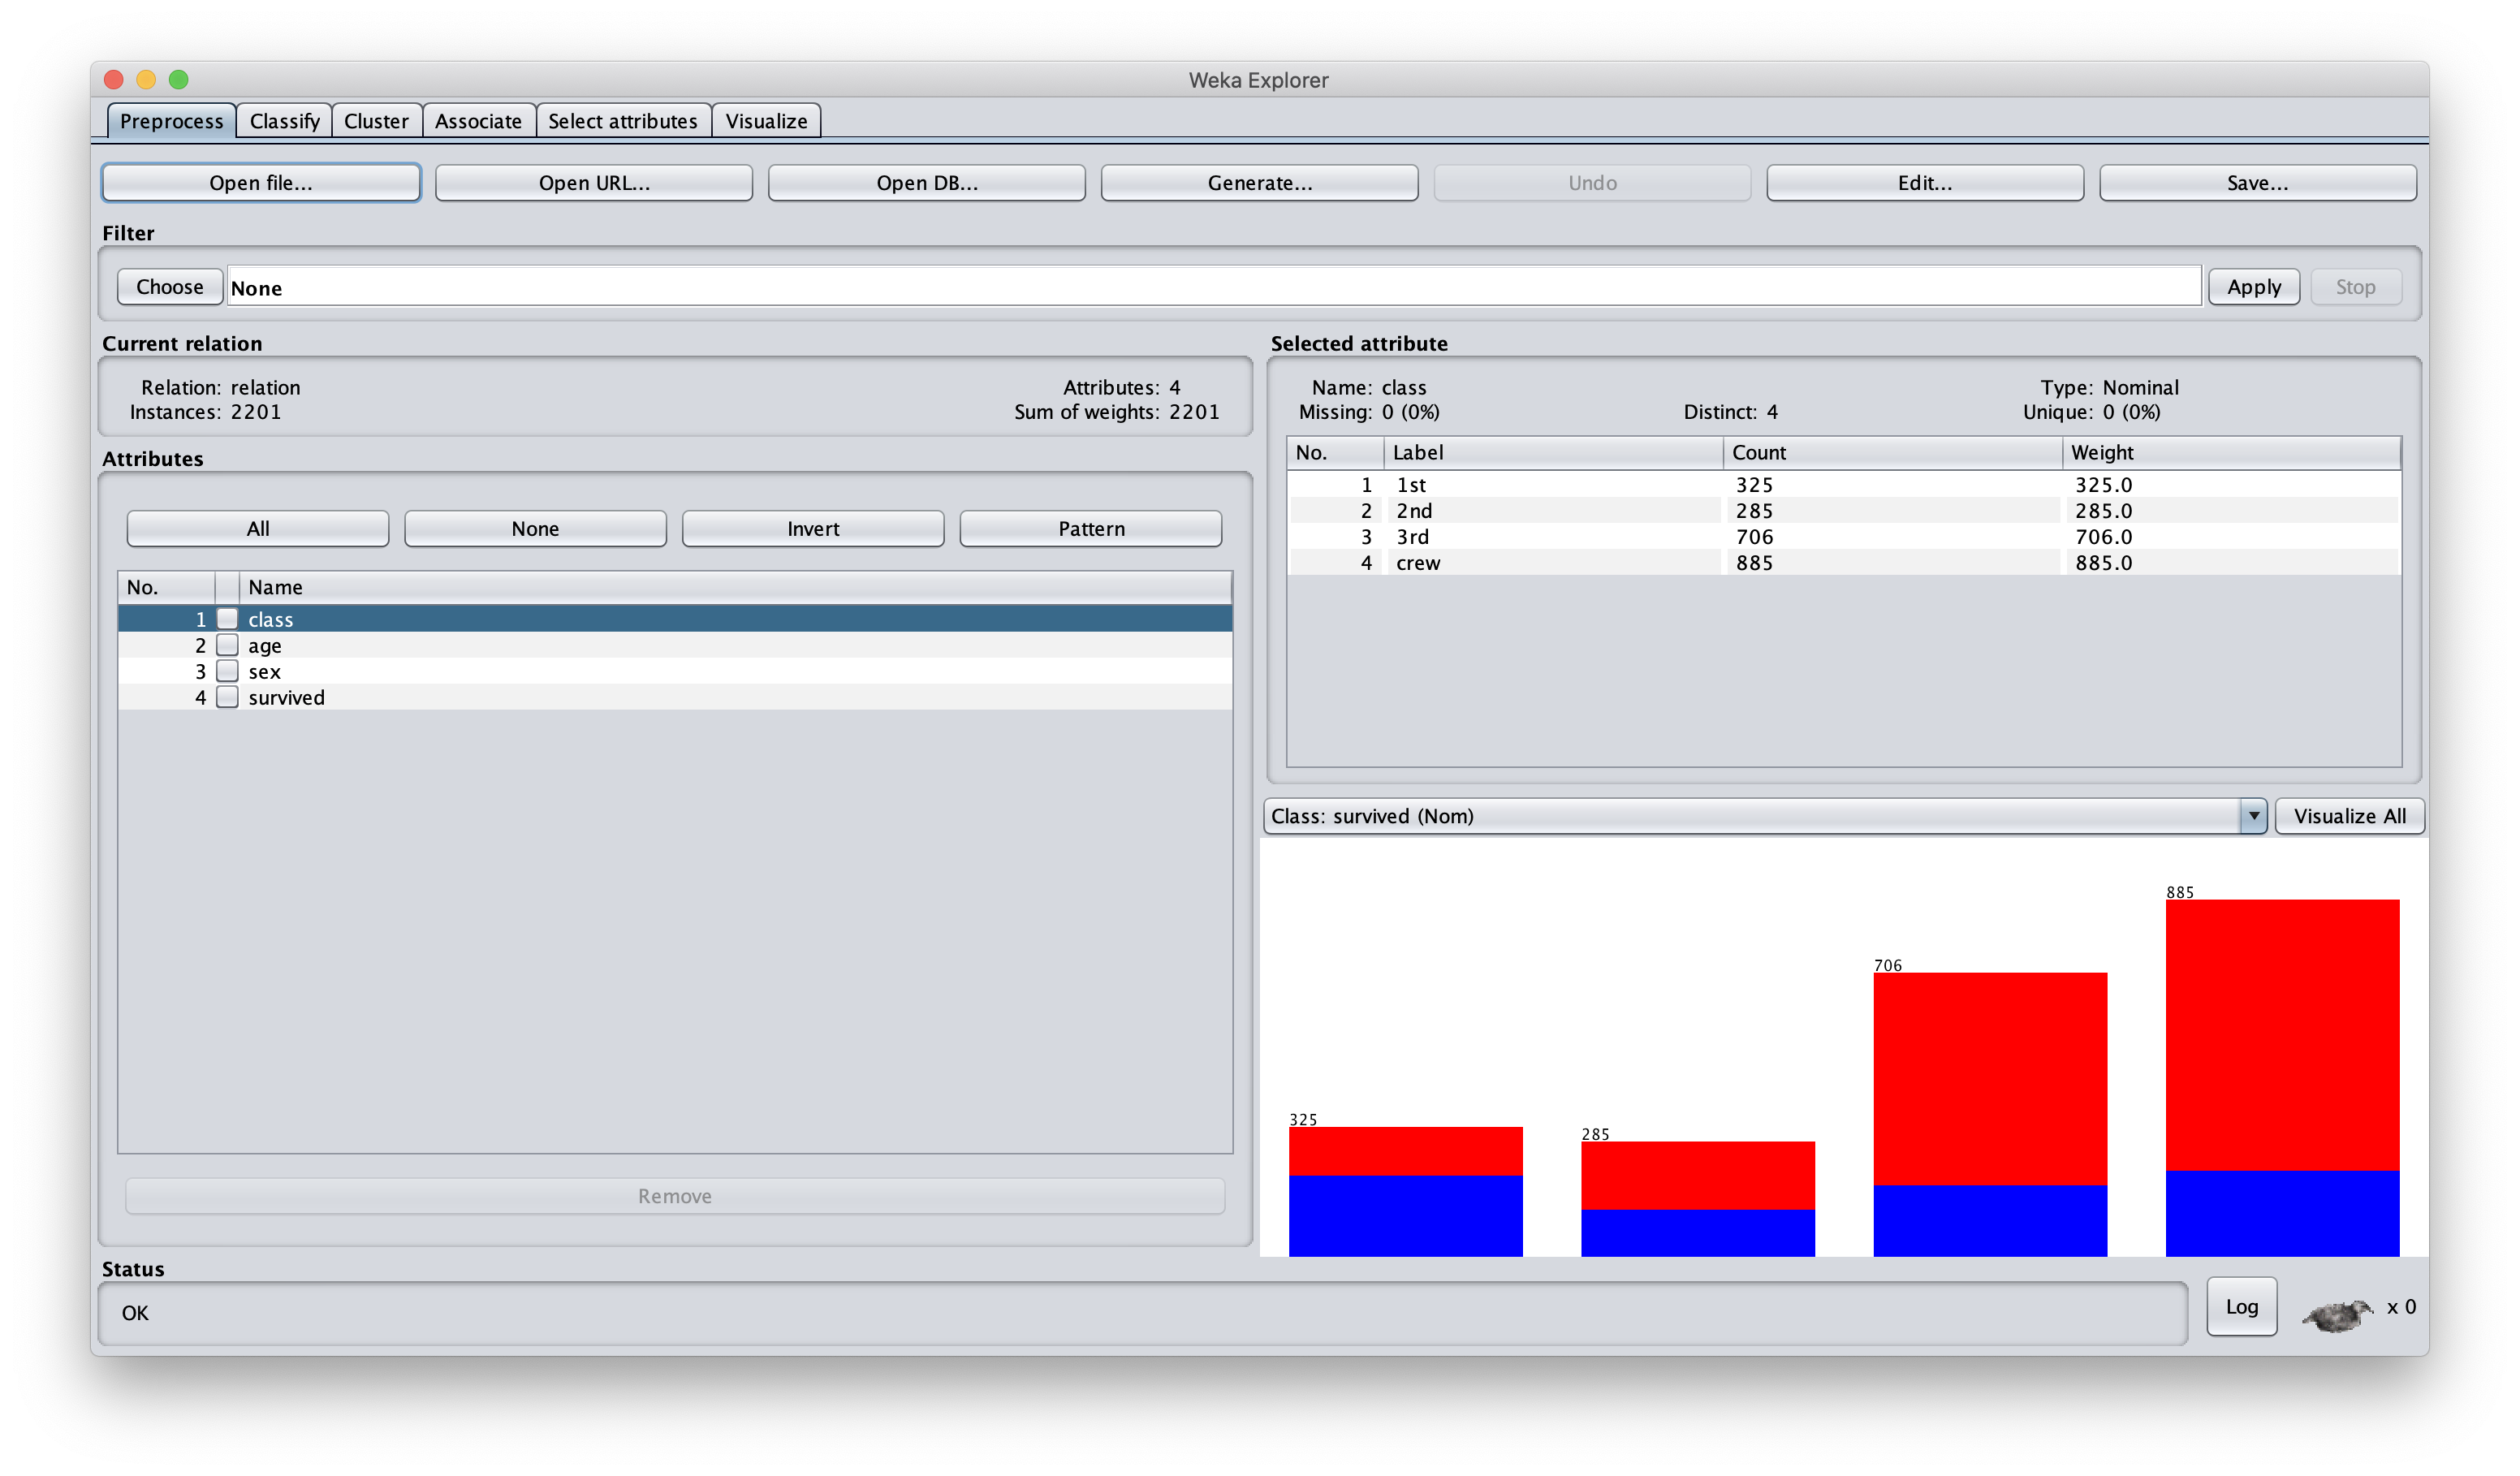
\includegraphics[scale=0.3]{Captura_1_2.png}
	\end{center}
\caption{características del dataset.}
\label{Captura_1_2}
\end{figure}

\part ¿Puede L(1) tomar un valor mayor que 10? Explica de manera teórica que eso no es posible y compruébalo experimentalmente.

L(1) no puede tomar un valor mayor que 10. El número de conjuntos de ítems de tamaño 1, como máximo podrá ser igual a 9. Ya que, como máximo, el número de conjuntos de ítems de tamaño 1, cuenta con los diferentes valores de cada atributo del dataset. 

\newpage
En este caso, el dataset de Titanic, contiene 9 valores diferentes:

\begin{itemize}
	\item Class ("1st", "2nd", "3rd", "Crew")
	\item Age {"Adult", "Child"}
	\item Sex {"Male", "Female"}
	\item Survived {"Yes", "No"}
\end{itemize}

Para comprobarlo experimentalmente, el umbral de confianza debe ser igual a 1. (ver Figura \ref{Captura_1_3})

\begin{figure}[h]
	\centering
	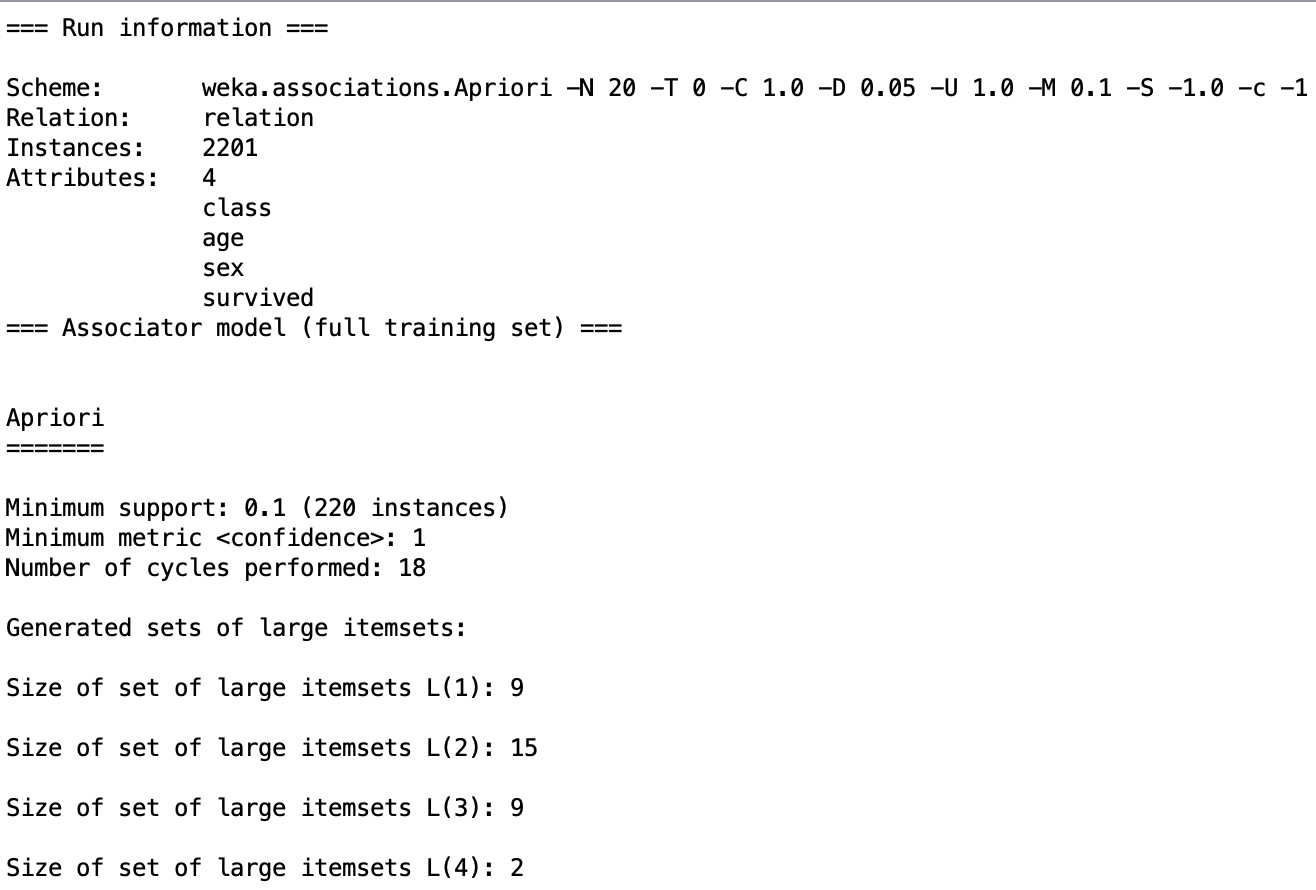
\includegraphics[scale=0.5]{Captura_1_3.png}
	\caption{soporte = 0.1 y confianza = 1.}
	\label{Captura_1_3}
\end{figure}

\end{parts}

% Pregunta 2
{\question Además de los valores de soporte, el algoritmo Apriori de Weka nos permite utilizar diferentes umbrales de soporte y confianza. Responde a las siguientes preguntas, utilizando capturas de pantalla y explicando los resultados de manera clara y concisa:}

\begin{parts}
\part ¿Es posible que una regla tenga un valor de soporte inferior a su confianza? Explica porqué y demuéstralo experimentalmente.

Es posible que una regla aparezca con poca frecuencia en el dataset pero que los conjuntos de ítems que la forman estén muy correlacionados. Para explicar el porqué y demostrarlo nos ayudaremos de la métrica \textit{lift} (mejora de la confianza). La métrica lift mide la relación del valor del soporte observado con el valor del soporte esperado de los conjuntos de ítems que forman cada regla, si esos conjuntos son independientes. Los conjuntos de ítems estarán positivamente correlacionados si el valor de lift es superior a 1, si el valor de lift es inferior a 1 estarán negativamente correlacionados, y si el valor de lift es igual a 1, estarán equilibradamente correlacionados.

En este caso, si una regla puede tener un valor de soporte inferior a su confianza, el valor de lift será superior a uno y nos indicará que el conjunto de ítems que forman la regla aparecen una cantidad de veces superior a lo esperado, por lo que se puede intuir que la regla hace que los conjuntos de ítems que la forman aparezcan más de lo normal. 

Por ejemplo, en la regla,

\vspace{2mm}
\textit{class=crew 885 ==$>$ age=adult 885    $<$conf:(1)$>$ lift:(1.05) lev:(0.02) [43] conv:(43.83)}
\vspace{2mm}

vemos que el número de instancias que aparecen en el dataset los conjuntos de ítems de la regla es elevado (885), y el valor de lift es superior a uno. Eso nos permite saber que existen muchas co-ocurrencias entre estos dos conjuntos y que la regla será potencialmente útil para predecir. Concretamente, ha resultado ser la regla número uno (Ver Figura \ref{Captura_1_4}).

\begin{figure}[h]
	\centering
	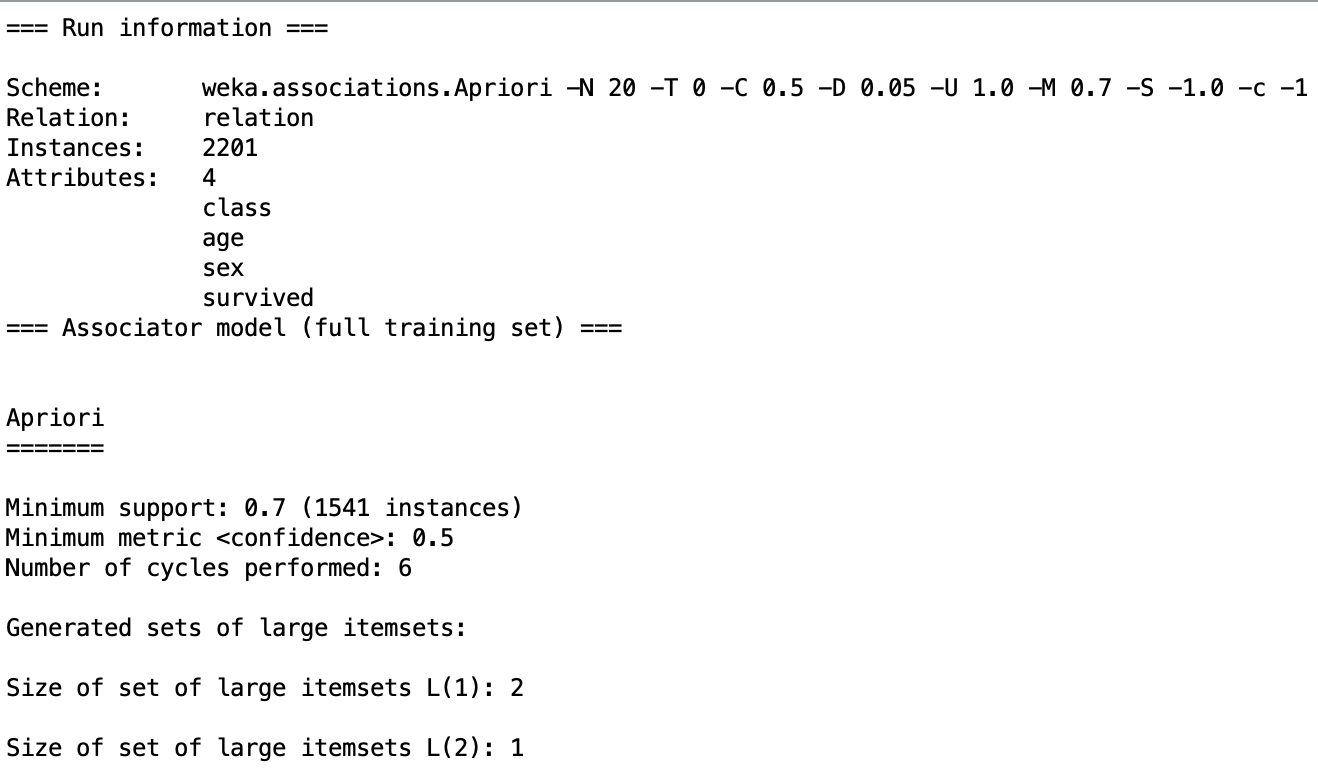
\includegraphics[scale=0.45]{Captura_1_4.png}
	\caption{soporte inferior a confianza.}
	\label{Captura_1_4}
\end{figure}

\part ¿Es posible que una regla tenga un valor de confianza inferior a su suporte? Explica porqué y demuéstralo experimentalmente.

También es posible que una regla aparezca con mucha frecuencia en el dataset pero que los conjuntos de ítems que la forman estén poco correlacionados. En este caso, el valor de lift será inferior a uno y nos indicará que el conjunto de ítems que forman la regla aparecen una cantidad de veces inferior a lo esperado, por lo que se puede intuir que la regla hace que los conjuntos de ítems que la forman aparezcan menos de lo normal. 

Por ejemplo, la regla,

\vspace{2mm}
\textit{class=3rd 706 ==$>$ age=adult sex=male 462    $<$conf:(0.65)$>$ lift:(0.86) lev:(-0.03) [-72] conv:(0.7)}
\vspace{2mm}

vemos que el número de instancias que aparecen en el dataset los conjuntos de datos no es tan elevado (706 y 462). Además no aparecen con la misma frecuencia en el dataset y el valor de lift es inferior a uno. Eso nos permite saber que existen menos co-ocurrencias entre los conjuntos de ítems que forman la regla y que esto tiene un efecto implicativo negativo. Potencialmente la regla no será tan útil para predecir. Y concretamente, ha resultado ser la regla número cuarenta (Ver Figura \ref{Captura_1_5}).

\begin{figure}[h]
	\centering
	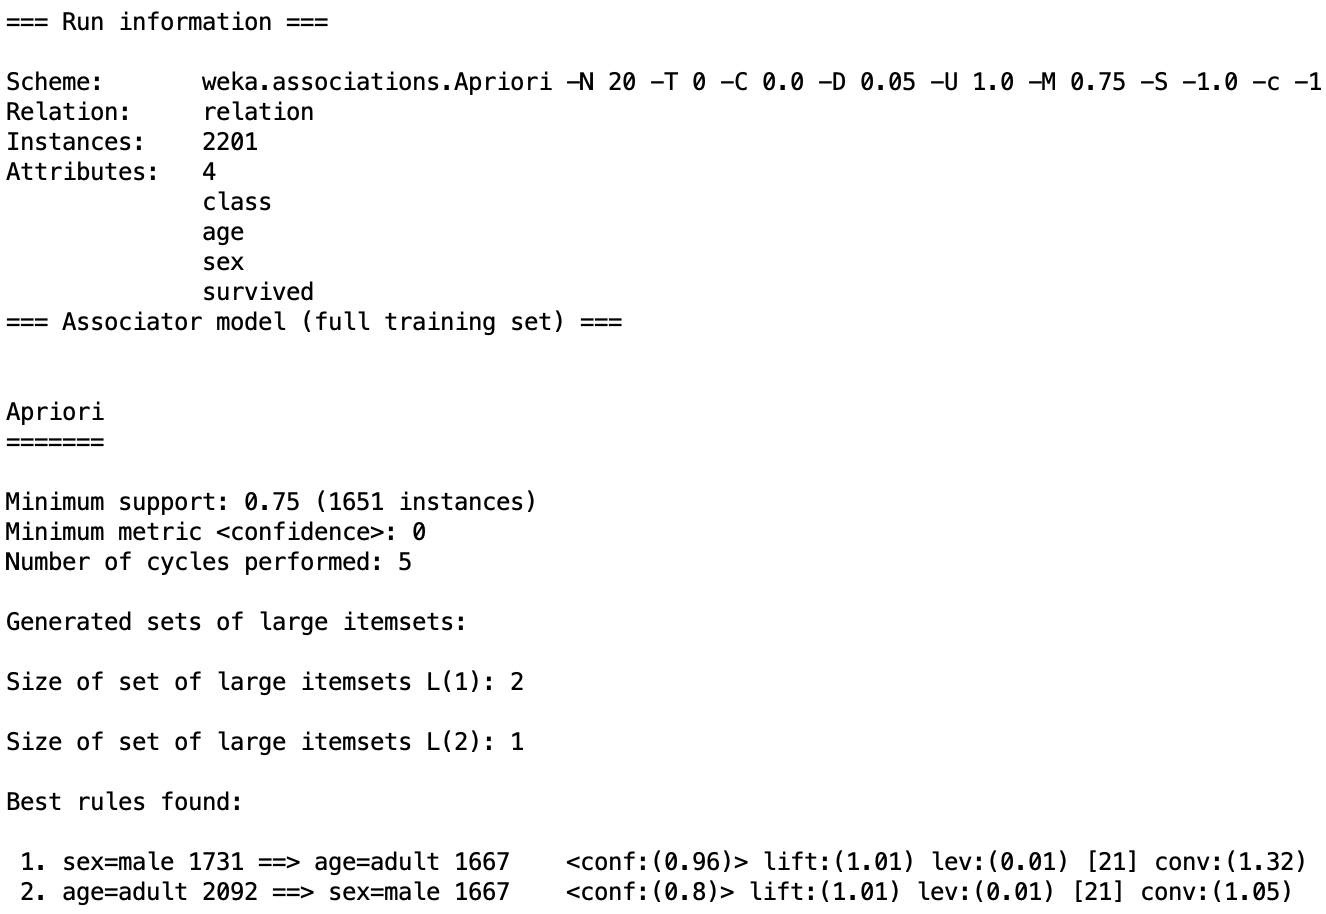
\includegraphics[scale=0.45]{Captura_1_5.png}
	\caption{soporte superior a confianza.}
	\label{Captura_1_5}
\end{figure}

\part La variación del umbral de confianza (dado un umbral fijo de soporte) no afecta a los conjuntos L(1)... L(4). ¿Por qué?
\end{parts}

Porqué la variación del umbral de confianza mide la relación entre los conjuntos de ítems que forman las reglas y no la frecuencia de aparición de los conjuntos de ítems de las reglas, eso lo hace el umbral de soporte. Y como los conjuntos de ítems L(1)... L(4) representan el número de apariciones de conjuntos de ítems según su tamaño dentro del dataset, el umbral de soporte les afectará. Por ejemplo, si el umbral de soporte es pequeño, Weka nos mostrará pocos conjuntos de ítems que no aparecen en el dataset, al contrario cuando el umbral del soporte sea mayor.

% Pregunta 3
{\question Usaremos ahora, 0.75 como valor mínimo de soporte y de confianza 0.00. Comprobamos que obtenemos dos reglas de asociación, sin embargo, L(2) es 1. ¿Qué quiere decir esto? ¿A qué corresponde L(2)? ¿Qué itemset representa?}

Esto quiere decir que el algoritmo Apriori ha encontrado un conjunto de ítems de tamaño dos que no forma parte de ninguna regla, ya que los conjuntos de ítems que la forman no están correlacionados. Este conjunto representa las personas adultas (hombres o mujeres). Ver Figura \ref{Captura_1_6}.

\begin{figure}[h]
	\centering
	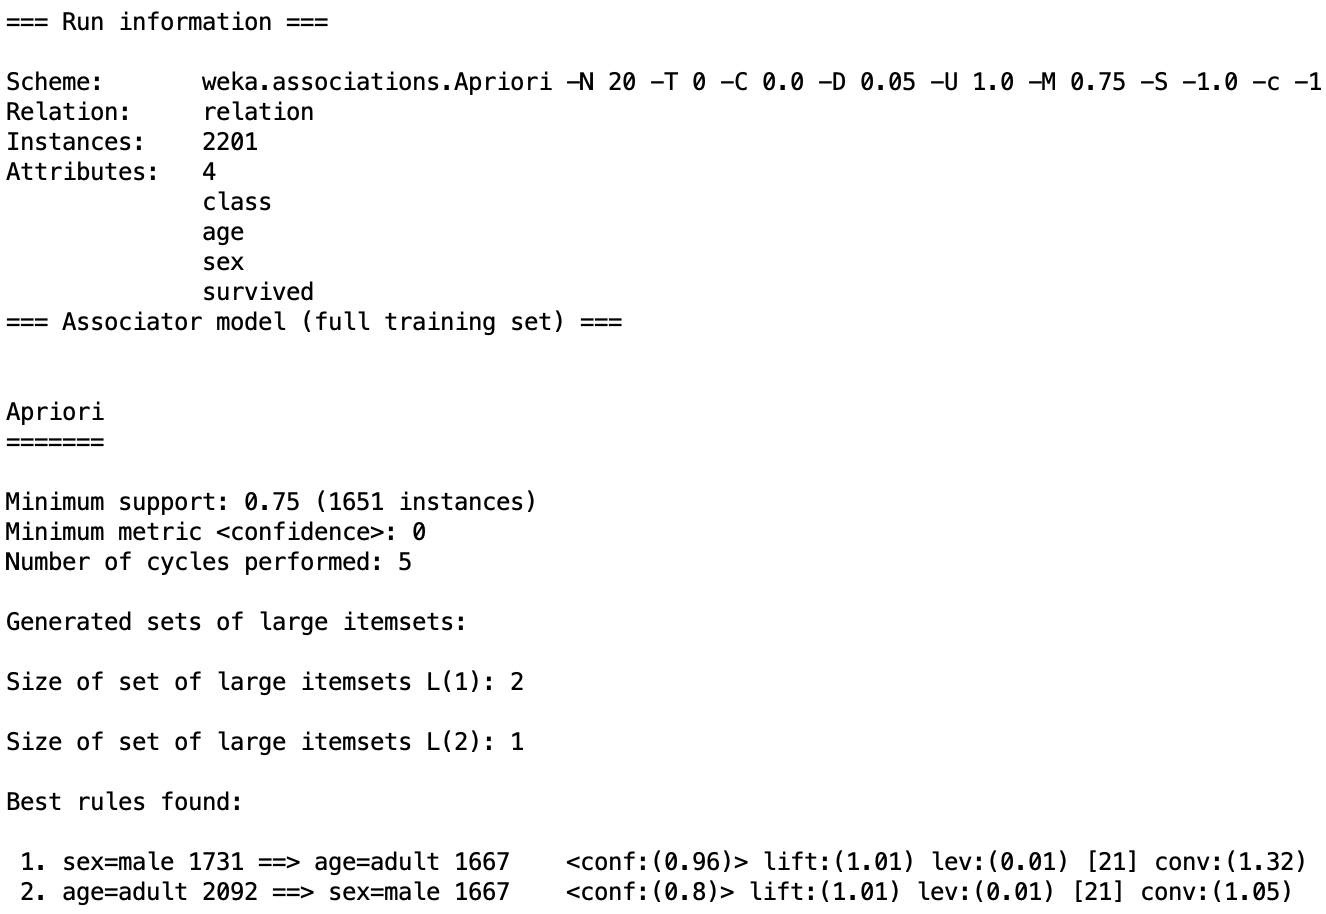
\includegraphics[scale=0.5]{Captura_1_6.png}
	\caption{soporte = 0.75 y confianza = 0.}
	\label{Captura_1_6}
\end{figure}

\newpage
% Pregunta 4
{\question Analiza el conjunto de reglas que salen al aplicar diferentes umbrales de soporte y confianza. Coge una regla, la que veas más interesante, y coméntala. Explica sus valores de métricas y qué representan, y el significado de la regla, es decir, el conocimiento que te aporta dicha regla.}

Después de aplicar diferentes umbrales de soporte y confianza la regla elegida es la siguiente:

\begin{figure}[h]
	\centering
	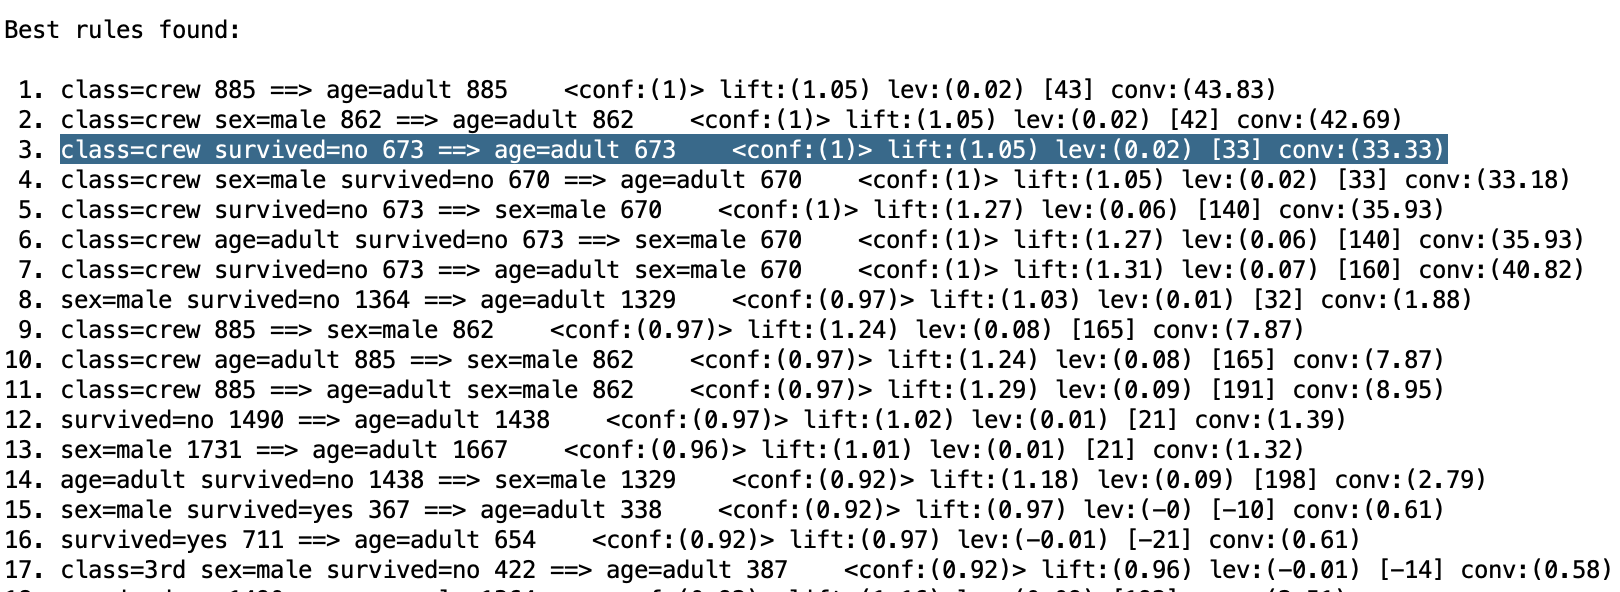
\includegraphics[scale=0.5]{Captura_1_7.png}
	\caption{tripulación que no sobrevivió.}
	\label{Captura_1_7}
\end{figure}

Esta regla nos indica las personas adultas de la tripulación que no sobrevivieron al naufragio del Titanic. Las métricas que podemos observar en ella son:

\begin{itemize}
	\item La confianza con valor igual a 1. Lo que significa que para el 100\% de las transacciones del dataset que contienen los conjuntos de ítems que forman la regla, la regla se cumplirá siempre. Es decir, siempre que una persona de la tripulación no haya sobrevivido, esta persona será adulta. Esto es cierto, porqué no existe ningún miembro de la tripulación que fuera un niño.
	\item La mejora de la confianza o lift, con valor igual a 1.05. Como se ha comentado anteriormente, si el valor de lift es superior a 1, permite saber que hay muchas co-ocurrencias entre los conjuntos de ítems que forman la regla y que dependen unas de ellas. Eso hace que la regla sea potencialmente útil para predecir y extraer información del dataset muy relevante. Podríamos decir que la mayoría de las personas que no sobrevivieron fueron personas de la tripulación.
	\item La influencia o \textit{leverage}, con valor igual a 0.02. Es una métrica muy parecida a lift, pero mide la proporción de que los conjuntos de ítems de las reglas no estén correlacionados entre sí. En este caso, su valor es muy pequeño. Eso quiere decir que los conjuntos de ítems que forman la regla están muy correlacionados. Así, si el valor de lift es alto el valor de leverage tiende a ser bajo, y al revés.
	\item La convicción o \textit{conviction}, con valor igual a 33.33. Es una métrica que nos indica el grado de implicación de la regla dentro del dataset. Y el grado de implicación en este caso es alto y puede señalar un aspecto relevante del dataset. Muchas de las personas que no sobrevivieron fueron personas adultas de la tripulación, concretamente un 33.33\%.
\end{itemize}

\end{questions}

\end{document}
